\documentclass{beamer}

\mode<presentation>
{
  \usetheme{CambridgeUS}
  \setbeamercovered{transparent}
}

\usepackage[english]{babel}
\usepackage[latin1]{inputenc}
\usepackage{times}
\usepackage[T1]{fontenc} 
% Or whatever. Note that the encoding and the font should match. If T1
% does not look nice, try deleting the line with the fontenc.
\usepackage{amsmath}

\newcommand{\linespace}{\vskip 0.25cm}

\definecolor{MyForestGreen}{rgb}{0,0.7,0} 
\newcommand{\tableemph}[1]{{#1}}
\newcommand{\tablewin}[1]{\tableemph{#1}}
\newcommand{\tablemid}[1]{\tableemph{#1}}
\newcommand{\tablelose}[1]{\tableemph{#1}}

\definecolor{MyLightGray}{rgb}{0.6,0.6,0.6}
\newcommand{\tabletie}[1]{\color{MyLightGray} {#1}}

% The text in square brackets is the short version of your title and will be used in the
% header/footer depending on your theme.
\title[CNNs in Medical Imaging]{Convolutional Neural Networks \\ in Medical Imaging}

% Sub-titles are optional - uncomment and edit the next line if you want one.
% \subtitle{Why does sub-tree crossover work?} 

% The text in square brackets is the short version of your name(s) and will be used in the
% header/footer depending on your theme.
\author[Finzel]{Mitchell Finzel}

% The text in square brackets is the short version of your institution and will be used in the
% header/footer depending on your theme.
\institute[U of Minn, Morris]
{
  Division of Science and Mathematics \\
  University of Minnesota, Morris \\
  Morris, Minnesota, USA
}

% The text in square brackets is the short version of the date if you need that.
\date[April '17] % (optional)
{15 April 2017, \\ Senior Seminar Conference}

% Delete this, if you do not want the table of contents to pop up at
% the beginning of each subsection:
\AtBeginSection[]
{
  \begin{frame}<beamer>
    \frametitle{Outline}
    \tableofcontents[currentsection, hideothersubsections]
  \end{frame}
}

\begin{document}

\begin{frame}
  \titlepage
\end{frame}

% For a 20-25 minute senior seminar talk you probably want something like:
% - Two or three major sections (other than the summary).
% - At *most* three subsections per section.
% - Talk about 30s to 2min per frame. So there should probably be between
%   15 and 30 frames, all told.

\section*{Overview}

\begin{frame}
  \frametitle{Outline}
  \tableofcontents[hideallsubsections]
  \begin{itemize}
  	\item Introduction - A brief look at CNNs and biological image segmentation in a broader scope.
  	\item Background - Information about basic structural concepts for CNNs
  	\item Methods used by Havaei, et al.
  	\item Methods used by Kamnitsas, et al.
  	\item Results
  	\item Conclusions
  \end{itemize}
\end{frame}

\subsection*{Background}

\begin{frame}
  \frametitle{Kernels}
  
  \begin{columns}
  \begin{column}{0.6\textwidth}
  \begin{itemize}
	\item Kernels, neurons and filters are interchangeable names
	\item Kernels are an array based representation of image features
  \end{itemize}
  \end{column}
  \begin{column}{0.4\textwidth}
   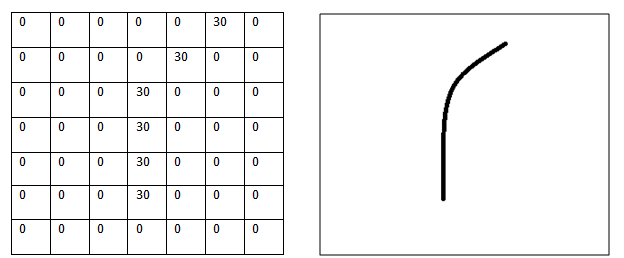
\includegraphics[width=0.95\textwidth]{Filter.png}
       \\
    \only{\tiny{Kernel \\ \url{https://adeshpande3.github.io/} }}
  \end{column}
  \end{columns}
\end{frame}

\begin{frame}
	\frametitle{Convolutional Layers}
	
  \begin{columns}
  \begin{column}{0.6\textwidth}
  \begin{itemize}
	\item Convolutional Layers are where CNNs get their name
	\item Every CNN starts with a convolutional layer
	\item The Kernel slides or "convolves" around the input image
	\item The results of the convolutions are stored in the feature map
  \end{itemize}
  \end{column}
  \begin{column}{0.4\textwidth}
   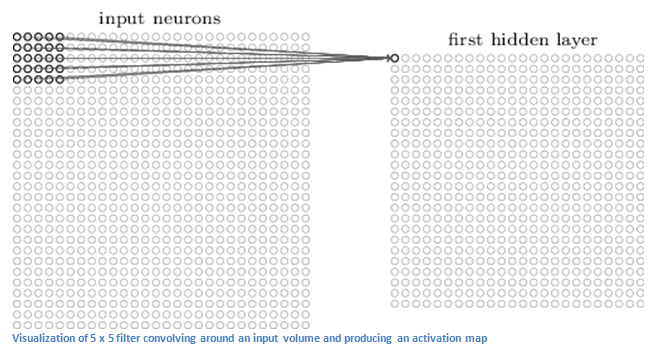
\includegraphics[width=0.95\textwidth]{ActivationMap.png}
       \\
    \only{\tiny{Feature Map \\ \url{https://adeshpande3.github.io/} }}
  \end{column}
  \end{columns}
\end{frame}


\end{document}


